\documentclass[
  oneside,
  degree=bachelor,
  fullwidthstop=false,
  fontset=fandol,
  times=false,
  minted=true,
  biblatex=true,
]{tongjithesis}

\tjbibresource{bib/note.bib}

\begin{document}

% ============================================================
%  封面信息
% ============================================================
\school{计算机科学与技术学院}
\major{软件工程（软件工作）}
\student{2251321}{徐嘉豪}
\thesistitle{一款轻量级实时数字协作白板系统}{设计与开发}
\thesistitleeng{A Lightweight Real-time Digital Collaborative Whiteboard System}{Design and Development}
\thesisadvisor{张晶\quad 指导教师}
\thesisdate{\the\year}{\the\month}{\the\day} % 使用当前日期; 也可以自定义日期

% ============================================================
%  信息说明页
% ============================================================

% 成果类型：design（毕业设计）或 thesis（毕业论文）
\infotype{thesis}

% 内容简述（请用300字以内简要概述）
\infoabstract{%
QuickBoard 是一个“打开即用”的在线协作白板系统，面向课堂讨论与远程协作场景，目标是在无需注册的前提下，实现秒级创建/加入房间与稳定的多人实时绘制体验。系统前端基于 Vue3 与 Fabric 实现可编辑画布，提供选择、画笔、形状、橡皮与导出等能力；后端基于 Node.js 与 Socket.IO 完成房间管理与实时消息通信，并采用服务端权威裁决与增量同步策略减少冲突与回滚；同时接入独立 OCR 服务识别数学公式并在前端以 KaTeX 渲染与可编辑流程实现“识别—确认—插入—编辑”闭环。本文给出需求分析、总体架构与关键实现，并通过单元测试与构建验证及场景化功能测试评估系统可用性与稳定性。
}

% 毕业设计：图纸数量与正文字数（成果类型为 design 时填写，两者须同时填写）
% \infodrawings{5}
% \infowordcount{15000}

% 毕业论文：正文总字数（成果类型为 thesis 时填写）
\infothesiswords{8000}

% 随附资料（每条用 \item 开头；不填则显示空白行）
\infomaterials{
  \item 程序源代码（前端、后端与 OCR 服务）；
  \item 测试报告与构建报告（\texttt{doc/test\_reports}）。
}

\MakeCover
\cleardoublepage
\MakeInfoPage
\cleardoublepage

\frontmatter
\MakeAbstract{
    本文设计并实现了一款轻量级实时数字协作白板系统 QuickBoard，面向课堂讨论与远程协作场景，强调无需注册、秒级创建/加入房间的使用体验。系统前端基于 Vue3 与 Fabric 实现可编辑画布，提供选择、画笔、形状、橡皮、文本与导出等基础能力；后端基于 Node.js 与 Socket.IO 实现房间管理与实时消息通信，并采用服务端权威裁决与增量同步策略减少冲突与回滚；同时接入独立 OCR 服务完成数学公式识别，并在前端以 KaTeX 渲染与可编辑弹层实现“识别—确认—插入—二次编辑”的闭环体验。本文围绕需求分析、系统设计与关键实现展开，给出核心模块的数据流与接口定义，并通过单元测试、构建验证与典型协作场景测试对系统可用性与稳定性进行评估。结果表明，该系统能够满足轻量协作白板的主要需求，并为后续扩展更丰富的图形组件与协作能力提供了可扩展的实现基础。
}{在线白板，实时协作，Socket.IO，OCR，KaTeX}

\MakeAbstractEng{
    This thesis designs and implements QuickBoard, a lightweight real-time digital collaborative whiteboard for classroom discussions and remote teamwork. It emphasizes instant room creation/joining without sign-up. The frontend is built with Vue 3 and Fabric to provide essential drawing capabilities such as selection, pen, shapes, eraser, text, and export. The backend is implemented with Node.js and Socket.IO for room management and real-time messaging, and adopts a server-authoritative decision with incremental synchronization to reduce conflicts and rollback issues. In addition, a standalone OCR service is integrated to recognize mathematical expressions, and KaTeX-based rendering with an editable workflow enables a complete loop of recognition, confirmation, insertion, and further editing. This thesis presents requirement analysis, system design, and key implementations with clarified data flows and interfaces, and evaluates availability and stability through unit tests, production builds, and scenario-based collaborative tests. The results show that the system meets the core needs of a lightweight collaborative whiteboard and provides a scalable foundation for future extensions.
}{online whiteboard, real-time collaboration, Socket.IO, OCR, KaTeX}


\clearpage
\tableofcontents
% \listoffigures   % 插图清单（根据需要取消注释）
% \listoftables    % 表格清单（根据需要取消注释）
\cleardoublepage

\mainmatter
\chapter{绪论}\label{chap:introduction}

\section{研究背景}
随着在线教学、远程会议与跨地域协作的常态化，团队在讨论过程中的“即时表达”需求不断增强。相较于传统文档协作，白板能够更自然地承载草图、流程图与推导过程，尤其适合用于快速构思与讲解。在实际使用中，用户往往希望在尽量低的门槛下迅速进入协作状态，即“打开即可用、创建即可分享、加入即可同步”。

现有白板产品在功能完整性与使用成本之间通常存在取舍：平台化产品往往引入账号体系、团队空间与复杂权限配置；而极简产品虽然上手快，但在多人同步、网络波动与跨端一致性方面可能出现体验问题。基于上述背景，设计并实现一个聚焦核心协作链路、以房间化方式降低使用成本的在线白板系统具有现实意义。

\section{研究意义}
本课题的意义主要体现在以下方面：
\begin{itemize}
  \item \textbf{工程实践价值}：综合应用现代前端框架、图形渲染与实时通信技术，完成从需求到交付的系统实现与验证闭环。
  \item \textbf{协作体验价值}：以房间号与邀请链接为核心入口，降低进入协作的操作成本，提升“创建—分享—加入”的效率。
  \item \textbf{可扩展性价值}：通过清晰的模块边界与同步策略，为后续扩展更多图形组件、增强一致性与持久化能力提供基础。
\end{itemize}

\section{国内外研究与现状}
在线白板的发展经历了从单机绘图工具到 Web 化协作平台的演进。产品形态上，一类系统强调极简与快速进入，适合轻量协作；另一类系统更强调团队化与流程化能力，适用于复杂项目管理。技术路线方面，前端多采用基于 Canvas 或 WebGL 的图形渲染方案，协作层多基于 WebSocket 类实时通信实现状态广播与同步；在冲突处理上，常见策略包括按时间戳的最后写入优先、服务端权威裁决以及更复杂的 CRDT/OT 等一致性算法。

在教学与工程讨论场景中，快速创建房间并共享给同伴、在网络波动下仍能保持基本可用，是用户体验的关键。QuickBoard 选择以“轻量房间协作 + 必要绘图工具 + 数学公式识别闭环”为目标，不追求平台化功能，但重点保证核心链路的稳定与快速。

\section{本文主要工作}
围绕 QuickBoard 在线白板系统，本文完成的主要工作包括：
\begin{itemize}
  \item 设计并实现基于房间的白板协作入口，支持创建房间、加入房间与最近房间管理；
  \item 实现基于 Node.js 与 Socket.IO 的实时协作通信，并采用服务端权威裁决与增量同步策略提升一致性体验；
  \item 集成 OCR 服务实现数学公式识别，并在前端实现渲染与二次编辑流程；
  \item 通过单元测试与构建验证等方式对系统进行验证，并在交互与渲染侧进行针对性优化以提升稳定性与响应速度。
\end{itemize}

\section{论文结构}
本文结构安排如下：第 \ref{chap:tech} 章介绍系统实现所涉及的关键技术；第 \ref{chap:req} 章进行需求分析；第 \ref{chap:design} 章给出系统总体架构与模块设计；第 \ref{chap:impl} 章阐述关键实现；第 \ref{chap:eval} 章对系统进行测试与评估；第 \ref{chap:conclusion} 章给出总结与展望。


\chapter{相关技术}\label{chap:tech}

本章介绍 QuickBoard 系统实现所涉及的关键技术与选型依据，涵盖前端框架与构建工具、画布渲染、实时通信、公式渲染与 OCR 服务等。

\section{前端框架与工程化}
\subsection{Vue3 与 Vite}
QuickBoard 前端采用 Vue3 进行组件化开发，通过响应式状态管理实现工具状态、房间信息与 UI 交互的联动。构建工具选择 Vite，以更快的开发热更新与生产构建能力提升迭代效率。该组合能够在保证工程可维护性的同时降低构建与调试成本。\cite{vue3,vite}

\subsection{Tailwind CSS}
项目使用 Tailwind CSS 进行样式组织，通过原子类组合实现按钮、输入框、卡片等基础样式，并结合少量自定义样式定义动效与背景纹理，从而在不引入复杂设计系统的情况下满足极简风格需求。

\section{画布渲染与交互：Fabric.js}
在线白板的核心是“可编辑画布”。QuickBoard 使用 Fabric.js 封装原生 Canvas 提供的绘制能力，将图形元素抽象为对象（Object），并提供选择、拖拽、缩放、命中检测等交互能力。相比直接操作 Canvas API，Fabric 更易于管理多对象场景，并支持序列化与反序列化，便于协作同步与导出。

在性能方面，项目通过视口裁剪与对象缓存等策略降低不必要的重绘开销，同时在选中对象时关闭缓存以避免编辑过程中的视觉滞后。\cite{fabricjs}

\subsection{Canvas 性能特征与优化方向}
Canvas 渲染通常运行在单线程主线程上，渲染与事件处理共享同一执行栈。当对象数量增大时，性能瓶颈往往来自三个方面：对象遍历成本（每帧遍历大量对象）、不可见对象绘制成本（视口外对象仍参与绘制）、以及重复绘制成本（静态对象每帧被重复光栅化）。因此，优化方向也相对明确：通过视口裁剪跳过不可见对象；通过对象缓存对静态对象复用位图；通过减少无效重绘与合并绘制批次降低每帧开销。QuickBoard 的渲染优化围绕上述方向展开，并以基准测试量化优化前后的平均渲染耗时变化。

\section{实时通信：Socket.IO}
实时协作需要低延迟、双向通信与房间管理机制。QuickBoard 后端基于 Socket.IO 提供房间语义、断线重连与事件广播能力；前端通过 Socket.IO Client 进行连接、加入房间、发送绘制事件与接收他人更新。相较于直接使用原生 WebSocket，Socket.IO 在工程实践中提供了更完善的事件模型与连接管理能力，降低了实现复杂度。\cite{socketio}

\subsection{WebSocket 协议基础}
浏览器与服务端的实时通信通常建立在 WebSocket 协议之上。WebSocket 通过一次 HTTP 握手升级为全双工长连接，减少轮询带来的额外开销，并能以较低延迟推送事件\cite{rfc6455}。在白板协作场景中，绘制增量、对齐事件与成员状态变更都具有“频繁、小包、时效敏感”的特点，长连接模型能够更好地匹配这种事件流。

\section{同步策略与冲突处理}
多人编辑不可避免地带来并发冲突与消息乱序问题。QuickBoard 采用“服务端权威裁决 + 增量同步”的设计思想：客户端发送操作增量，服务端对关键字段进行最后写入优先（LWW）裁决后再广播被接受的变更；同时维护房间版本号与增量日志，使新加入或断线重连的客户端可以通过版本差量补齐状态，必要时再回退到全量快照。该策略在工程复杂度与一致性体验之间取得平衡，适合毕业设计的轻量协作场景。

\subsection{OT 与 CRDT 的对比与取舍}
协作一致性领域常见的两条技术路线为 OT 与 CRDT。OT 通过对并发操作进行转换来保持意图，并在早期协同编辑系统中得到广泛应用\cite{sun_ellis_1998}；CRDT 则以“可交换、可合并的数据结构”为核心，天然支持最终一致性与离线合并\cite{shapiro_rr7506_2011}。二者的共同点是能够在并发修改下保证收敛，但在工程实现成本、调试复杂度与数据模型适配性方面存在差异。

QuickBoard 的白板状态以“图形对象集合”为核心：对象数量多、字段多、交互频繁，且系统定位为短会话协作。若引入通用 CRDT 框架，需要为对象集合与字段更新设计更复杂的可交换结构，并处理 tombstone、压缩与持久化等配套问题；若采用 OT，需要为各类对象操作定义转换规则并在服务端维护操作序列。综合考虑毕业设计的交付周期与可解释性要求，QuickBoard 采用更轻量的字段级 LWW，并以服务端权威裁决降低分叉概率，通过版本补包与快照兜底保证最终收敛。

\subsection{逻辑时钟与 LWW 合并}
在 LWW 策略中，“写入的新旧”需要一个可比较的时间戳。若直接使用客户端物理时间，可能因时钟偏差导致误判；因此工程上常使用逻辑时钟为更新分配单调递增的序号，并在接收远端更新后对本地逻辑时钟进行追赶。该思路与分布式系统中对事件顺序的经典讨论一致\cite{lamport_1978}。QuickBoard 将时间戳关联到对象字段，以字段级别进行比较与合并，从而避免“整对象覆盖”带来的误更新与额外网络开销。

\section{公式渲染与编辑：KaTeX}
为了支持数学公式的高质量排版，项目在前端使用 KaTeX 将 LaTeX 字符串渲染为数学公式。与将 LaTeX 作为纯文本绘制到 Canvas 不同，QuickBoard 采用渲染层叠加的方式显示公式，并提供双击编辑、实时预览与确认插入流程，从而提升可读性与可编辑性。\cite{katex}

\subsection{可编辑渲染与对象模型的协调}
在白板对象模型中，公式既需要像普通对象一样被选择、移动、缩放与序列化，又需要在视觉上以高质量排版呈现。QuickBoard 将公式的“数据层”和“显示层”分离：数据层以 LaTeX 字符串形式作为对象字段参与同步与持久化；显示层由 KaTeX 在前端渲染生成可读的排版结果。该分离使得跨端同步时传输的是稳定的文本表示，而不是与分辨率或字体强相关的位图；同时也为“二次编辑”提供了自然入口——用户编辑的是 LaTeX 数据，渲染层随之更新。

\section{数学公式识别：OCR 服务}
QuickBoard 的公式识别功能采用独立 OCR 服务实现。前端对白板选区进行截图并发送到后端接口，后端将请求转发至 OCR 服务并返回识别结果。OCR 服务侧对输入图像进行必要的预处理（如尺寸对齐、内容裁剪、反色/二值化等），并在结果为空或包含噪声时进行清洗与回退尝试，最终以统一格式返回 LaTeX 或错误信息。该“前端采集—后端代理—OCR 服务识别”的三段式架构便于部署与调试，也降低了前端复杂度。\cite{fastapi}

\subsection{预处理的重要性}
数学 OCR 的输入具有明显的“非规范性”：笔迹粗细与倾斜程度差异大，背景可能包含网格或色块，框选区域可能过紧导致字符被裁剪，也可能过松引入大量噪声。若直接将原始截图输入识别模型，空结果或错误结果的概率显著上升。因此，工程实践中通常需要在服务端加入预处理步骤，例如对输入尺寸进行对齐、对深色背景做反色、对前景进行二值化或增强，并在必要时构造多种预处理候选以提升命中概率。QuickBoard 将预处理与失败回退作为 OCR 链路的核心组成部分，并通过统一错误码与 traceId 让失败原因具备可定位性。

\subsection{错误码与可定位性}
与“返回空字符串”相比，统一错误码能够把失败原因分类为可操作的工程问题：例如超时（资源或网络问题）、空结果（输入质量或模型能力问题）、坏图（裁剪或编码问题）。traceId 则提供跨组件追踪的锚点，使一次识别请求可以在前端日志、后端代理与 OCR 服务端日志中被关联。通过错误码与 traceId，OCR 评估可以从“好不好用”的主观感受，落到“哪些失败类型占主导、如何改进”的工程分析路径上。

\section{极简白板产品参考}
为提升“快速进入、低干扰”的首屏体验，首页信息架构参考了 Excalidraw 等极简白板产品的设计取向，并结合房间化协作入口进行本地化改造。\cite{excalidraw}

\chapter{需求分析}\label{chap:req}

本章从用户角色与典型场景出发，给出 QuickBoard 的功能需求与非功能需求，并明确系统边界与约束。

\section{用户角色与使用场景}
系统主要面向无需注册的访客用户，典型场景包括：课堂讨论中的板书推导、线上会议中的流程图与方案讨论、远程结对时的草图沟通等。该类场景的共同点是：进入速度优先、协作过程对稳定性敏感、对复杂权限与长期项目管理需求较弱。

\section{功能需求}
\subsection{房间与入口}
\begin{itemize}
  \item \textbf{创建房间}：用户点击创建按钮后，系统生成房间号并进入白板页面。
  \item \textbf{加入房间}：用户可输入房间号或粘贴邀请链接进入对应房间；输入非法时应给出明确提示。
  \item \textbf{最近房间}：记录用户最近进入的房间列表，支持一键进入与移除记录。
\end{itemize}

\subsection{白板编辑}
\begin{itemize}
  \item \textbf{基础工具}：选择、画笔、形状（如矩形/圆形）、橡皮擦、文本等。
  \item \textbf{画布操作}：平移与缩放、对象选择与移动、删除与基本属性调整。
  \item \textbf{导出能力}：支持将白板内容导出为图片或数据文件，便于保存与分享。
\end{itemize}

\subsection{实时协作}
\begin{itemize}
  \item \textbf{多人同步}：同一房间的多个用户可看到彼此的绘制结果与对象变更。
  \item \textbf{重连与补包}：断线后能够自动重连，并尽量恢复到最新状态，避免刷新回滚。
\end{itemize}

\subsection{公式识别与编辑}
\begin{itemize}
  \item \textbf{公式识别}：用户框选区域后发送至 OCR 服务识别，返回 LaTeX。
  \item \textbf{确认插入}：识别结果需支持用户确认后再插入画布，避免误识别污染画布。
  \item \textbf{二次编辑}：插入后的公式可双击进入编辑，实时预览渲染效果并更新画布显示。
\end{itemize}

\section{典型用例}
为使需求具备可验证性，本课题将核心流程抽象为代表性用例，并在第 \ref{chap:eval} 章通过实验与场景测试进行验证。

\subsection{用例A：创建房间并分享}
\textbf{前置条件}：用户打开系统首页。\par
\textbf{基本流程}：点击创建按钮生成房间号并进入画板；页面展示可分享链接/房间号；其他用户通过链接或房间号加入同一房间。\par
\textbf{验收要点}：进入路径短、房间号易输入、分享后可直接进入同一协作域。

\subsection{用例B：多人实时绘制与撤销重做}
\textbf{前置条件}：两名或以上用户处于同一房间。\par
\textbf{基本流程}：用户 A 绘制路径/形状/文本并产生对象增量；服务端裁决后广播；用户 B 端出现一致对象；撤销/重做操作同步生效。\par
\textbf{验收要点}：对象集合一致、撤销重做行为多端一致。

\subsection{用例C：断线重连对齐}
\textbf{前置条件}：房间存在持续编辑且某客户端发生断线。\par
\textbf{基本流程}：客户端恢复连接后 join-room 携带 clientVersion；服务端根据 roomVersion 与增量日志能力发送 sync-delta 或 sync-state；客户端对齐后继续协作。\par
\textbf{验收要点}：断线窗口结束后最终收敛，且对齐路径明确。

\subsection{用例D：公式识别与插入}
\textbf{前置条件}：用户在画布上写出公式或导入手写内容。\par
\textbf{基本流程}：框选区域并发起识别；返回 LaTeX 或错误码；用户确认/修改后插入为公式对象；远端同步显示并可再次编辑。\par
\textbf{验收要点}：成功路径闭环；失败路径提示明确；可通过 traceId 与可选 debug 图定位失败原因。

\section{非功能需求}
\subsection{可用性与易用性}
系统应保证首屏聚焦主任务（创建/加入房间），并在操作反馈上保持清晰。关键流程应尽量减少弹窗与中断式交互，错误提示应直观且可恢复。

\subsection{实时性与一致性}
在网络条件正常时，多人协作的更新应具有较低延迟；在并发冲突与消息乱序场景下，系统需提供可解释的裁决策略，并尽量避免状态回滚。

\subsection{稳定性与性能}
系统需在常见浏览器环境下稳定运行。白板渲染应在多对象场景下保持可交互性，公式识别在失败时应及时返回并允许用户继续操作。

\subsection{可验证指标}
为提高论文论证的可复核性，本课题将部分非功能需求转化为可量化指标：
\begin{itemize}
  \item \textbf{最终收敛}：在丢包与断线场景下，多端结束时的权威对象集合应收敛到单一版本（结束时哈希种类数为 1）。
  \item \textbf{渲染性能}：在 5000 对象规模的基准场景下，启用视口裁剪与对象缓存后平均渲染耗时应明显下降。
  \item \textbf{过程降载}：在持续书写输入下，过程预览链路应显著降低消息数量，并保证结束信号正确。
\end{itemize}

\begin{table}[htbp]
  \centering
  \caption{核心需求与验证方式}\label{tab:req-verify}
  \renewcommand{\arraystretch}{1.35}
  \begin{tabular}{lll}
    \toprule
    \textbf{需求项} & \textbf{验证方式} & \textbf{证据来源} \\
    \midrule
    弱网最终收敛 & 一致性对照实验 & \texttt{doc/test\_reports/quickboard\_sync\_benchmark} \\
    大对象渲染可用 & 渲染性能基准 & \texttt{doc/test\_reports/quickboard\_render\_perf} \\
    过程预览不拥塞 & Ghost Brush 降载统计 & \texttt{doc/test\_reports/quickboard\_ghost\_brush} \\
    OCR 可用且可定位 & 场景测试 + 错误码/traceId & 项目日志与截图 \\
    \bottomrule
  \end{tabular}
\end{table}

\subsection{安全性与隐私}
系统默认无需用户身份信息，房间链接作为共享入口应避免泄露敏感数据；对于本地保存的最近房间记录，应明确其仅存储在浏览器本地存储中。

\section{约束与边界}
本项目聚焦本科毕业设计的实现与验证，不包含账号体系、复杂权限管理与长期存储的团队空间等平台化能力。协作一致性以“工程可用与体验稳定”为优先目标，不追求强一致性下的复杂冲突合并算法。

\chapter{系统设计}\label{chap:design}

本章给出 QuickBoard 的总体架构、模块划分与主要数据流，重点说明“房间入口—白板协作—公式识别”三条主链路的设计取舍。

\section{总体架构}
QuickBoard 采用前后端分离与服务拆分的架构，整体可分为三部分：前端 Web 应用、后端协作服务与 OCR 服务。前端负责 UI、画布渲染与交互；后端负责房间管理、实时消息与状态同步；OCR 服务负责图像预处理与公式识别推理。该拆分方式便于独立部署与调试，也降低了前端的计算与依赖复杂度。

\begin{figure}[htbp]
  \centering
  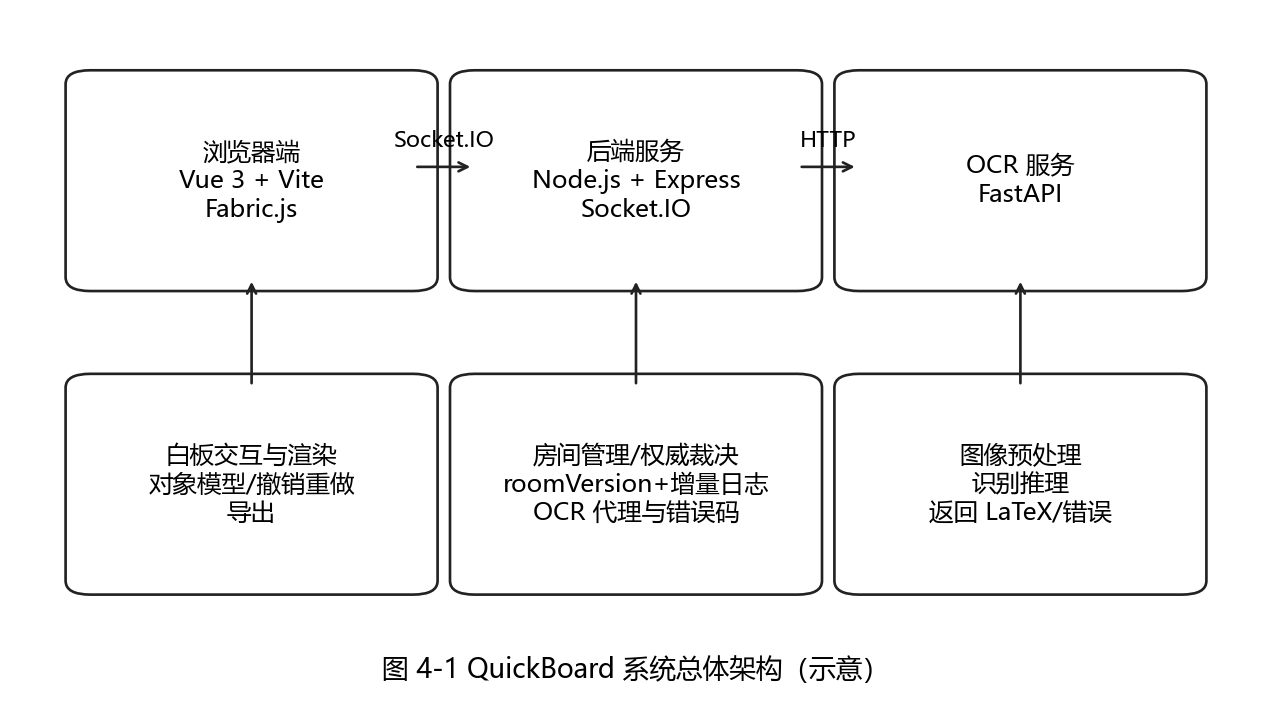
\includegraphics[width=0.92\linewidth]{figures/arch_quickboard.png}
  \caption{QuickBoard 系统总体架构}\label{fig:arch}
\end{figure}

\begin{figure}[htbp]
  \centering
  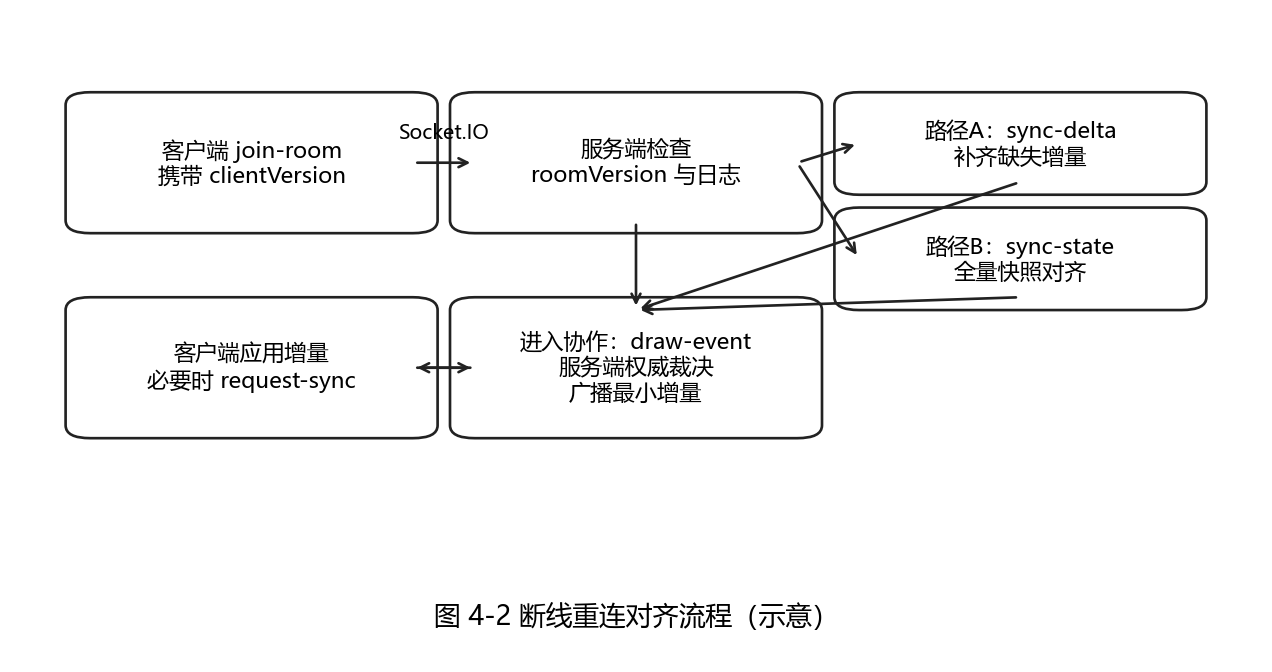
\includegraphics[width=0.92\linewidth]{figures/sync_flow.png}
  \caption{断线重连对齐流程示意}\label{fig:sync-flow}
\end{figure}

\section{模块划分}
\subsection{前端模块}
\begin{itemize}
  \item \textbf{首页模块}：提供创建房间、加入房间、最近房间管理等入口能力，并以极简布局聚焦主任务。
  \item \textbf{白板模块}：基于 Fabric.js 维护画布与对象模型，实现绘制、选择、形状、橡皮与导出等功能。
  \item \textbf{协作模块}：封装 Socket.IO 连接、房间加入、事件发送与接收，并处理断线重连与版本补包。
  \item \textbf{公式模块}：完成选区截图、识别请求、结果确认、KaTeX 渲染与双击编辑等流程。
\end{itemize}

\subsection{后端模块}
\begin{itemize}
  \item \textbf{房间管理}：维护房间生命周期与在线用户信息，支持空房间按 TTL 清理。
  \item \textbf{同步裁决}：对绘制事件进行服务端权威裁决，广播被接受的增量变更，并维护房间版本号与增量日志。
  \item \textbf{OCR 代理}：提供统一接口，将前端识别请求转发至 OCR 服务并规范化返回结构。
\end{itemize}

\subsection{OCR 服务模块}
\begin{itemize}
  \item \textbf{图像预处理}：对输入截图进行内容裁剪、尺寸对齐、反色/二值化等处理，提升识别成功率。
  \item \textbf{识别推理与回退}：优先调用公式识别模型，在失败或结果为空时对不同候选图像进行回退尝试。
  \item \textbf{结果清洗}：对输出 LaTeX 进行噪声清洗（如移除宏定义等），并对空结果统一返回错误码。
\end{itemize}

\section{关键数据流}
\subsection{创建/加入房间}
用户在首页创建房间后，前端生成房间号并进入白板页面；加入房间时，前端对输入进行归一化，支持从任意文本或链接中提取房间号并进入房间。后端根据房间号为连接分配房间上下文，并在必要时向客户端下发状态快照与增量补包。

\begin{figure}[htbp]
  \centering
  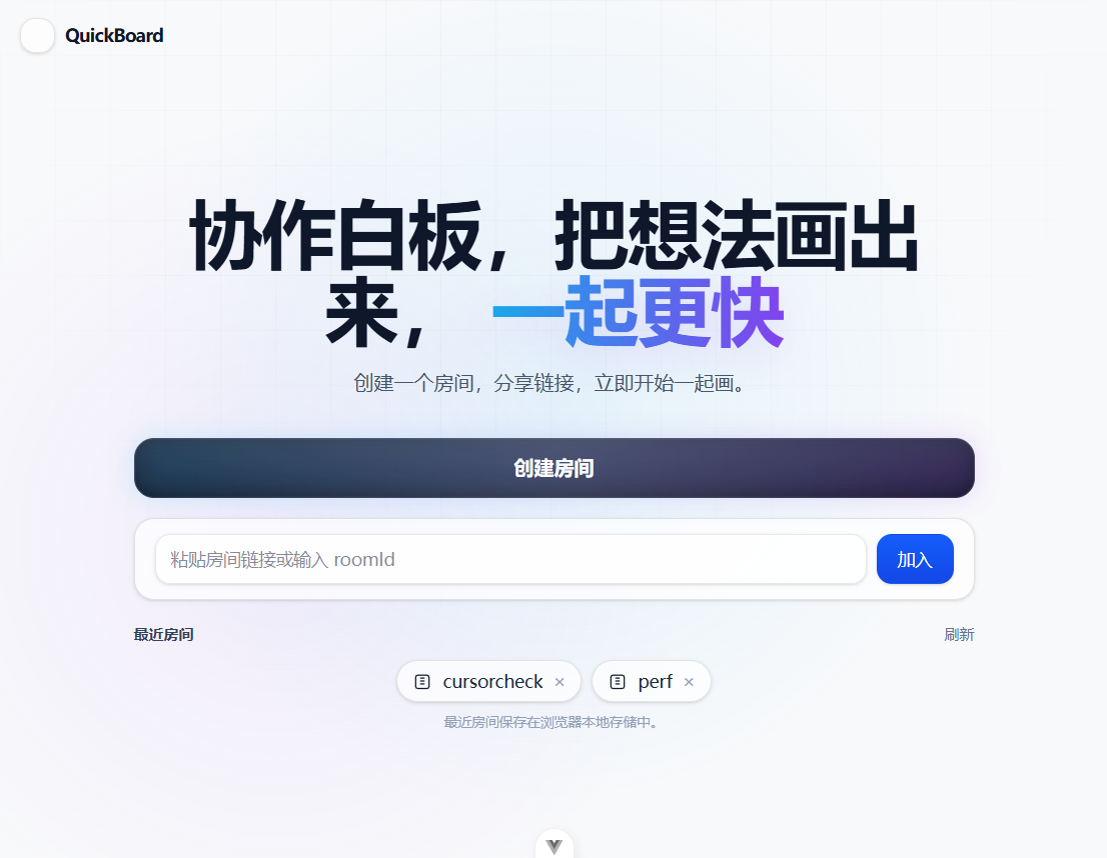
\includegraphics[width=0.9\linewidth]{figures/S1_home.png}
  \caption{系统首页入口示例}\label{fig:home}
\end{figure}

\subsection{白板协作同步}
前端对本地对象变更生成增量事件并发送至后端；后端对关键字段进行裁决后广播增量；客户端按版本号补齐缺失增量，必要时请求全量同步。该流程使协作在消息乱序与断线重连场景下仍能尽量保持一致。

\section{数据模型与事件设计}
\subsection{对象集合与字段时间戳}
系统以“对象集合”作为白板权威状态。每个对象由全局唯一 id 标识，对象属性被组织为 \texttt{data}（字段值）与 \texttt{timestamps}（字段时间戳）两部分。字段时间戳由客户端逻辑时钟生成，用于字段级 LWW 合并。删除通过写入 \texttt{\_deleted=true} 表示，并参与 LWW 比较，从而保证删除语义能够在对齐与乱序条件下自然获胜。

\subsection{核心事件}
表 \ref{tab:events} 汇总了系统主链路涉及的核心事件。事件命名与字段设计以“可解释、可对齐”为目标：对齐相关事件显式携带版本区间或权威快照，使断线窗口内的状态恢复路径明确。

\begin{table}[htbp]
  \centering
  \caption{系统核心事件汇总}\label{tab:events}
  \renewcommand{\arraystretch}{1.35}
  \begin{tabular}{lll}
    \toprule
    \textbf{事件} & \textbf{方向} & \textbf{语义与关键字段} \\
    \midrule
    join-room & C$\rightarrow$S & 加入房间，携带 userName、clientVersion \\
    draw-event & C$\rightarrow$S & 对象最小增量：id、data、timestamps \\
    sync-delta & S$\rightarrow$C & 版本补包：fromVersion、toVersion、deltas \\
    sync-state & S$\rightarrow$C & 权威快照：存活对象 + tombstones \\
    request-sync & C$\rightarrow$S & 主动请求对齐（触发快照下发） \\
    drawing-process & C$\leftrightarrow$S & 过程预览点批量（不进入权威状态） \\
    \bottomrule
  \end{tabular}
\end{table}

\subsection{公式识别与插入}
用户在白板上框选区域后，前端生成截图并调用后端识别接口；后端将请求转发至 OCR 服务并返回 LaTeX；前端展示识别结果并允许用户确认与编辑，确认后将公式作为可编辑对象插入画布并同步给其他协作者。

\subsection{错误码与 traceId 设计}
OCR 识别链路包含网络请求与模型推理，失败场景不可避免。为避免“失败无响应”或“无法解释原因”的体验断点，系统在设计上引入统一错误码与 traceId：错误码用于将失败类型显式分类（例如超时、输入无效、空结果、识别失败等），traceId 用于为一次识别请求提供跨组件关联的唯一标识。通过错误码与 traceId，前端能够给出一致且可恢复的提示，后端与 OCR 服务也能够对失败请求进行定位与排障，从而使公式能力具备工程可维护性。

\chapter{关键实现}\label{chap:impl}

本章结合项目实现，说明 QuickBoard 在“房间入口”“协作同步”“渲染优化”“公式识别与编辑”等方面的关键实现要点与工程取舍。

\section{房间号与入口归一化}
为了降低口述与输入成本，系统默认生成固定长度的纯数字房间号。首页加入房间支持直接输入房间号，也支持粘贴包含房间参数的链接或任意文本；前端在进入房间前对输入进行归一化，提取并校验房间号格式，从而减少用户在不同分享方式下的摩擦。

\subsection{最近房间与本地存储}
短会话协作具有“频繁进入同一房间或少量房间”的特点。为降低重复进入成本，前端将最近进入的房间号记录在浏览器本地存储，并在首页以列表形式展示，支持一键进入与移除记录。该设计不依赖账号体系即可实现轻量的“历史回访”，同时避免将房间记录写入服务端引入隐私与存储负担。

\subsection{房间生命周期与自动清理}
为了避免短会话结束后房间长期占用内存，后端实现空房间 TTL 机制：当房间人数为 0 且超过一定时间窗口后进行清理，并以固定间隔扫描回收。该机制与短会话场景的时间分布匹配，能够在不引入复杂持久化的前提下控制资源占用，并减少服务端长期运行时的状态堆积风险。

\section{服务端权威裁决与版本补包}
多人协作场景中，客户端操作可能乱序到达或重复投递。QuickBoard 将同步裁决放在服务端执行：客户端发送增量事件后，服务端根据对象级最后写入优先（LWW）策略决定是否接受并广播；同时维护房间版本号与增量日志。客户端加入房间时携带自身版本号，优先通过差量接口补齐缺失增量，必要时再回退到全量快照。该设计可以有效降低“刷新回滚”与“大包同步”的概率。

\subsection{字段级 LWW 与最小增量广播}
为避免“整对象覆盖”带来的误更新，服务端以字段粒度执行 LWW 裁决：仅当 incoming 的字段时间戳大于服务端权威状态中对应字段时间戳时才接受该字段更新。裁决后服务端广播被接受字段集合构成的最小增量，使房间内所有客户端接收一致的裁决结果，并减少网络与序列化开销。

\subsection{删除墓碑与对象复活防护}
在对象集合模型中，删除是不可逆语义。若删除仅以“本地移除对象”表达，则漏包客户端无法推断对象已被删除，旧修改事件晚到时还可能导致对象复活。QuickBoard 将删除表示为字段 \texttt{\_deleted=true} 并参与 LWW 合并：当 \texttt{\_deleted} 的时间戳更“新”时，服务端拒绝所有旧字段更新。快照对齐时携带 tombstones，使漏包客户端在下一次对齐时也能完成删除收敛。

\subsection{版本补包与退化为全量快照}
后端维护 \texttt{roomVersion} 与增量日志 \texttt{deltaLogs}：每当一次增量被服务端裁决并接受，\texttt{roomVersion} 递增并记录该版本对应的最小增量。客户端重连时携带 \texttt{clientVersion}：若日志覆盖缺失区间则下发 \texttt{sync-delta} 补齐；若缺失跨度超出日志覆盖能力则退化为 \texttt{sync-state} 权威快照。该退化策略使对齐语义清晰并优先保证正确性。

\section{渲染性能优化}
Fabric 在对象数量较多时容易出现重绘压力。项目在默认配置下开启视口裁剪与对象缓存，对静态对象进行缓存，选中对象时临时关闭缓存以保证编辑反馈。开发环境中提供基准入口用于对比不同渲染策略的帧耗时表现，从而在不引入复杂性能工具的前提下完成可复现的优化验证。

\section{Ghost Brush：过程预览降载}
过程预览点位属于高频瞬时数据。若逐点发送，不仅会造成消息风暴，也会挤占权威增量的带宽，间接放大一致性风险。QuickBoard 将过程预览与权威状态解耦：预览点位先入队，按固定周期批量发送；当队列过长时进行均匀抽样但保留尾部点位；单条消息设置最大点数并在必要时拆包。服务端仅转发过程预览，不写入权威状态与快照路径，从而避免过程噪声污染一致性链路。

\section{公式识别链路}
\subsection{截图与裁剪}
公式识别采用“白板选区截图”的方式采集输入。为避免坐标系不一致导致的空白截图，前端基于底层 Canvas 像素进行裁剪并生成图像数据，再发送给后端识别接口。该方式能够更稳定地反映选区内容，并减少不同缩放状态下的误差。

\subsection{OCR 预处理与结果清洗}
OCR 服务对输入图像进行尺寸对齐与内容裁剪，并在暗底场景下自动反色，必要时进行二值化生成多候选输入以提升识别成功率。对于识别结果中的噪声（如宏定义片段），服务端进行清洗并在清洗后为空时继续回退，最终对空结果统一返回错误码，便于前端给出一致的错误提示。

\subsection{后端代理、错误码与 traceId}
为降低前端与 OCR 服务的耦合，QuickBoard 采用后端代理调用：前端只请求后端 \texttt{/api/recognize-math}，由后端转发至 OCR 服务并统一超时控制与错误映射。后端对失败场景返回统一错误码（例如 \texttt{TIMEOUT}、\texttt{BAD\_IMAGE}、\texttt{EMPTY\_LATEX}、\texttt{RECOGNIZE\_FAILED}），并生成 \texttt{traceId} 随响应返回，使一次识别请求在前端、后端与 OCR 服务之间可被定位与追踪。该机制将“识别失败”从不可解释的黑盒结果转化为可定位的工程问题，便于论文中的失败案例分析与后续迭代。

\section{公式渲染、确认插入与二次编辑}
识别得到的 LaTeX 并不直接以纯文本显示在画布上，而是通过 KaTeX 渲染为可读的数学公式。交互上，系统采用“识别后先确认再插入”的流程，避免误识别内容污染画布；插入后支持双击打开编辑弹层并实时预览渲染结果，确认后更新公式对象。为保证选框与实际渲染区域一致，公式对象在画布中的命中框会根据渲染尺寸进行补边与校正，从而提升选择与拖拽的可用性。

\subsection{超时控制与交互不中断}
公式识别涉及网络请求与模型推理，耗时具有不确定性。为避免识别请求长时间阻塞交互，前端在请求侧加入超时控制并支持中止，使用户在网络波动或服务端卡顿时仍可继续使用白板其他功能。后端同样设置请求超时并将失败映射为统一错误码，使“超时”在系统内部具有一致语义，便于前端提示与论文评估。

\subsection{对象序列化与一致显示}
为保证公式对象在多端显示一致，系统需要在对象序列化中携带与公式渲染相关的必要字段（例如 LaTeX 字符串与渲染尺寸信息）。在同步与对齐过程中，远端客户端根据这些字段重建对象，并使用同一渲染策略生成显示结果。相较于传输位图，传输 LaTeX 文本具有可编辑、体积小与跨分辨率稳定的优势；同时，命中框与边距的校正使选择、拖拽与缩放的交互体验更接近普通图形对象。

\chapter{测试与评估}\label{chap:eval}

本章围绕 QuickBoard 的核心目标进行测试与评估，重点验证：弱网与断线条件下的最终收敛、对象规模增长下的渲染性能，以及高频过程预览链路的网络降载效果。

\section{测试策略}
项目采用“单元测试 + 构建验证 + 可复核实验”的组合策略：
\begin{itemize}
  \item \textbf{单元测试}：覆盖协作通信、OCR 请求与裁剪、同步逻辑等核心模块，降低迭代带来的回归风险。
  \item \textbf{构建验证}：确保生产构建通过，避免仅开发环境可运行的问题。
  \item \textbf{可复核实验}：以一致性对照实验、渲染性能基准与降载统计测试对关键结论进行量化验证，并形成报告归档。
\end{itemize}

\section{单元测试与构建结果}
前端使用 Vitest 执行单元测试，并在每轮关键改动后执行构建验证。测试与构建输出以报告形式归档在 \texttt{doc/test\_reports}，便于回溯与论文撰写引用。

\begin{table}[htbp]
  \centering
  \caption{工程验证项汇总}\label{tab:verification}
  \renewcommand{\arraystretch}{1.35}
  \begin{tabular}{lll}
    \toprule
    \textbf{验证项} & \textbf{目的} & \textbf{结果} \\
    \midrule
    前端单元测试 & 覆盖核心逻辑、降低回归 & 通过 \\
    前端生产构建 & 确保可交付与可部署 & 通过 \\
    OCR 识别链路自检 & 验证预处理与返回格式 & 通过 \\
    \bottomrule
  \end{tabular}
\end{table}

\section{一致性对照实验：朴素广播 vs.\ LWW+补包}
为了验证弱网与断线场景下的最终收敛，采用 6 个客户端参与对照实验，并在接收侧引入丢包、延迟与抖动，同时对部分客户端施加断线窗口。评价指标选取“结束时哈希种类数”：对每个客户端结束时的权威对象集合做稳定序列化并计算哈希，统计不同哈希的数量。若系统最终一致，则哈希种类数应为 1；若出现分叉，则大于 1。

\begin{table}[htbp]
  \centering
  \caption{一致性对照实验关键结果}\label{tab:sync-benchmark}
  \renewcommand{\arraystretch}{1.35}
  \begin{tabular}{llll}
    \toprule
    \textbf{方案} & \textbf{网络扰动} & \textbf{断线窗口} & \textbf{结束时哈希种类数} \\
    \midrule
    朴素广播（naive） & recv drop=0.15, delay=90ms, jitter=140ms & clients=1,2 断线 2400ms & 6 \\
    LWW+补包（lww） & recv drop=0.15, delay=90ms, jitter=140ms & clients=1,2 断线 2400ms & 1 \\
    \bottomrule
  \end{tabular}
\end{table}

实验结果表明，朴素广播在丢包与断线条件下容易产生多版本分叉；采用服务端权威裁决、字段级 LWW 与版本补包后，系统能够收敛到单一权威状态。

\subsection{指标适用性讨论}
“结束时哈希种类数”用于回答“最终是否收敛到同一对象集合”这一问题，其优点是计算简单、可复核且不依赖主观判断。该指标的局限在于无法刻画收敛过程中的短时不一致程度，也无法表达意图保持等更强语义。考虑到 QuickBoard 的目标是短会话协作下的最终可用与可对齐，本章选择该指标与研究目标一致；若进一步研究意图保持或离线合并，则需要引入更细粒度的评估维度与数据结构支持。

\section{渲染性能基准：视口裁剪与对象缓存}
渲染基准在 6000$\times$6000 世界坐标内生成 5000 个对象，对比 Baseline（\texttt{skipOffscreen=false}, \texttt{objectCaching=false}）与 Optimized（\texttt{skipOffscreen=true}, \texttt{objectCaching=true}）两组配置，采样统计平均渲染耗时。基准结果来自项目归档报告。

\begin{table}[htbp]
  \centering
  \caption{渲染性能基准关键结果}\label{tab:render-benchmark}
  \renewcommand{\arraystretch}{1.35}
  \begin{tabular}{llll}
    \toprule
    \textbf{场景} & \textbf{Baseline avg render(ms)} & \textbf{Optimized avg render(ms)} & \textbf{可见对象占比} \\
    \midrule
    idle & 57.500 & 26.950 & $\approx 2.8\%$ \\
    pan & 52.275 & 16.225 & $\approx 2.8\%$ \\
    \bottomrule
  \end{tabular}
\end{table}

结果显示，在大对象规模场景下，视口裁剪显著降低参与绘制的对象数量；配合对象缓存可进一步降低重复绘制开销，从而明显降低平均渲染耗时。

\section{过程预览降载：Ghost Brush 统计验证}
过程预览属于高频瞬时数据，若逐点发送容易造成消息风暴并挤占权威增量带宽。针对 Ghost Brush 预览链路，采用算法级统计测试进行验证：10s 内以 4ms 采样（理论 2500 点），通过批处理与限包策略统计实际消息数。

\begin{table}[htbp]
  \centering
  \caption{Ghost Brush 降载测试关键结果}\label{tab:ghost-brush}
  \renewcommand{\arraystretch}{1.35}
  \begin{tabular}{llll}
    \toprule
    \textbf{采样点数（理论）} & \textbf{实际消息数} & \textbf{降载倍率} & \textbf{isEnd 次数} \\
    \midrule
    2500 & 279 & 8.96$\times$ & 1 \\
    \bottomrule
  \end{tabular}
\end{table}

统计结果表明，在保证轨迹连续展示与结束信号正确的前提下，批处理与限包机制能显著降低预览链路的消息数量，有助于降低多人同时书写时的网络压力。

\section{弱网实验入口示例}
图 \ref{fig:netsim} 展示了基于 URL 参数启用弱网扰动后的画板页面示例，用于说明实验条件可控。

\begin{figure}[htbp]
  \centering
  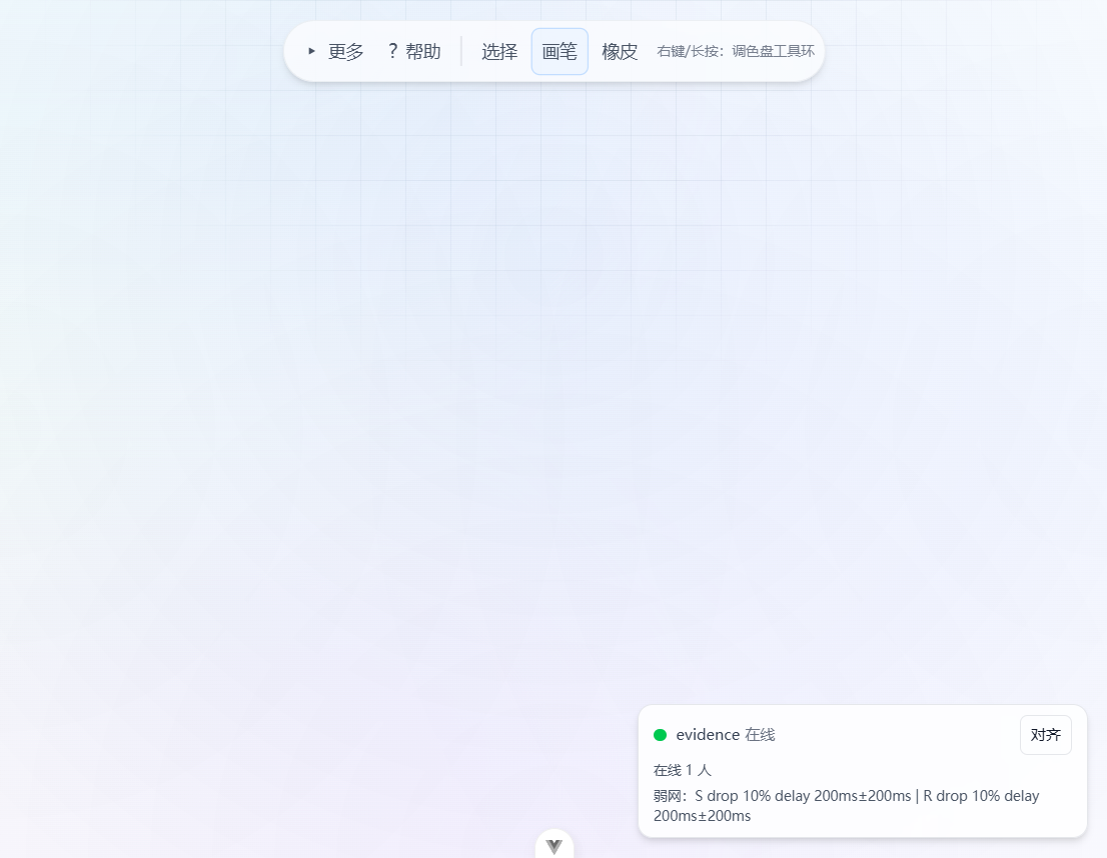
\includegraphics[width=0.92\linewidth]{figures/S3_netsim.png}
  \caption{弱网扰动参数开启示例}\label{fig:netsim}
\end{figure}

\section{威胁与局限性}
本课题的评估主要依赖工程脚本与自动化报告，能够保证可复核，但仍存在局限性：
\begin{itemize}
  \item \textbf{弱网扰动覆盖范围}：弱网模拟通过参数化丢包、延迟与抖动来构造网络扰动，无法完全覆盖真实移动网络中的复杂行为（例如链路层重传、突发拥塞与多路径切换）。
  \item \textbf{一致性语义范围}：字段级 LWW 强调最终收敛与实现可解释性，在极端并发同字段编辑时可能出现意图覆盖；本章指标侧重最终是否收敛，未对意图保持做进一步量化评估。
  \item \textbf{OCR 评估范围}：OCR 识别质量受输入分布与模型能力影响较大，本文强调可定位与可纠错的工程闭环，但未构建大规模数据集进行统计学评估。
\end{itemize}

\section{本章小结}
本章围绕 QuickBoard 的核心贡献给出三类可复核证据：一致性对照实验用于验证弱网与断线条件下的最终收敛；渲染基准用于量化对象规模增长下的性能改善；降载测试用于验证过程预览链路的消息量显著下降，并解释其对权威同步带宽的保护作用。通过将工程实现与评估证据绑定，论文论证从“实现了什么”进一步落到“为何有效、如何验证”。

\section{结果分析与不足}
从评估结果看，QuickBoard 的一致性策略在弱网与断线条件下能够实现最终收敛；渲染优化策略能够在对象规模较大时降低平均渲染耗时；过程预览降载能够显著降低消息量并减少对权威增量的干扰。其不足主要体现在：字段级 LWW 在极端并发同字段编辑时存在意图覆盖的语义取舍；OCR 识别质量仍受输入质量与场景分布影响；Canvas 渲染与对象模型在更大规模对象下仍可能出现性能瓶颈，后续可进一步探索更细粒度的渲染分层或 WebGL 路径。

\chapter{总结与展望}\label{chap:conclusion}

\section{工作总结}
本文围绕轻量级实时数字协作白板系统 QuickBoard 的设计与实现开展研究与工程实践，面向短会话协作场景，强调无需注册、快速创建/加入房间的使用体验。系统以三服务架构实现前端白板、后端协作与公式识别能力：前端基于 Vue~3 与 Fabric.js 提供对象级绘制与编辑；后端基于 Node.js（Express）与 Socket.IO 提供房间管理、实时事件分发与服务端权威裁决；OCR 服务基于 FastAPI 提供公式识别能力，并通过后端代理统一错误码与 traceId。

围绕本课题的核心工程风险点，本文完成并验证了以下工作：
\begin{itemize}
  \item \textbf{一致性策略落地}：采用服务端权威裁决与字段级 LWW 合并，结合 \texttt{roomVersion} 增量补包、快照兜底与手动对齐，形成可解释、可对齐的协作路径。评估表明该策略在丢包与断线窗口条件下能够实现最终收敛。
  \item \textbf{性能与降载优化}：在渲染侧通过视口裁剪与对象缓存降低大对象规模下的平均渲染耗时；在网络侧通过 Ghost Brush 将高频过程预览与权威状态解耦，并通过批处理与限包显著降低消息数量。
  \item \textbf{公式识别闭环}：实现“框选—裁剪—识别—确认插入—可编辑渲染”的闭环交互，并通过统一错误码、traceId 与可选 debug 回传提升失败可定位性，使公式能力在教学场景下具备可用性与可维护性。
\end{itemize}

综合测试与评估结果，QuickBoard 在工程复杂度可控的前提下实现了轻量协作白板的核心能力，并通过对照实验与基准测试提供了可复核的论证证据。

\section{后续展望}
后续工作可从以下方向进一步完善系统：
\begin{itemize}
  \item \textbf{一致性语义增强}：在保持系统可解释性的前提下，针对极端并发同字段编辑的意图保持进行增强；可探索在局部数据结构上引入 CRDT/OT 思路，或对高冲突对象设计更细粒度的数据模型。
  \item \textbf{持久化与历史回放}：在轻量前提下完善房间历史与版本回溯，使教学场景能够沉淀推导过程并支持复习与复盘。
  \item \textbf{权限与审计}：增加房间访问控制、主持人权限与操作审计，提升公开演示与课堂使用中的可控性。
  \item \textbf{OCR 量化评估与迭代}：构建更系统的样本集与量化指标（成功率、耗时分位数、可编辑率），并在不牺牲隐私与延迟的前提下持续提升识别质量。
  \item \textbf{跨端体验与可访问性}：完善快捷键、触控适配与视觉反馈，并针对移动端与不同分辨率设备持续优化交互与性能表现。
\end{itemize}


\makereferences

\appendix
\appendixsection{项目材料与报告索引}\label{sec:appendix-materials}

\appendixsubsection{项目结构说明}
QuickBoard 系统由前端、后端与 OCR 服务三部分组成：
\begin{itemize}
  \item \textbf{前端 Web 应用}：基于 Vue3 + Vite 与 Fabric.js，负责用户交互与画布渲染，包含白板编辑、房间入口与公式交互等模块。
  \item \textbf{后端协作服务}：基于 Node.js（Express）与 Socket.IO，负责房间管理、实时事件分发、同步裁决与版本对齐，并提供 OCR 请求的统一代理接口。
  \item \textbf{OCR 服务}：基于 FastAPI，负责图像预处理与数学公式识别推理，并输出可插入的 LaTeX 表达。
\end{itemize}

\appendixsubsection{验证材料说明}
为保证本文结论具有可复核性，关键改动均配套记录单元测试与构建验证结果；针对同步一致性、渲染性能与过程预览降载等关键结论，均记录实验参数、原始统计与结果摘要。相关验证材料随论文一并提交，便于复核与对照。

\appendixsubsection{开题报告图片复用}
\begin{figure}[htbp]
  \centering
  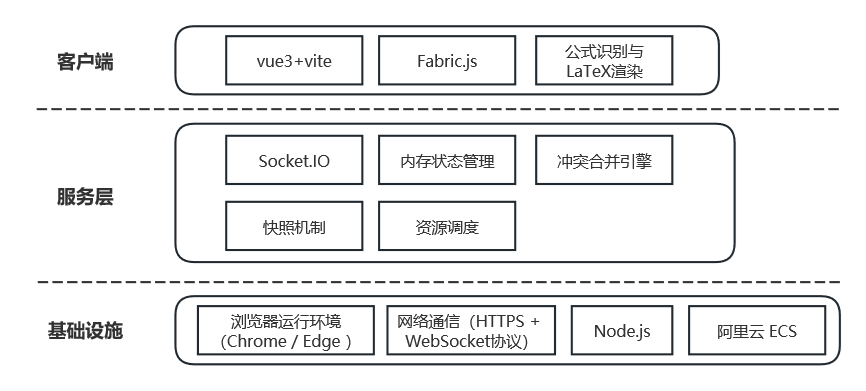
\includegraphics[width=0.92\linewidth]{figures/proposal_arch.png}
  \caption{开题报告阶段技术架构图（复用）}\label{fig:proposal-arch}
\end{figure}

\appendixsubsection{开题调研与需求分析补充}
本课题在开题阶段对短会话协作与教学场景的工具需求进行了归纳，并将需求收敛为“进入路径短、表达成本低、协作反馈及时、弱网可恢复、内容可沉淀”五类核心目标。其关键观点可概括如下。

\textbf{（1）进入路径短。} 短会话协作常发生在临时讨论与课堂推导中，参与者随时加入或离开。若系统依赖注册、团队空间配置或复杂权限设置，会显著增加进入成本并打断讨论节奏。因此系统入口优先提供创建/加入房间与复制分享链接，房间号采用纯数字便于口述与输入，最近房间用于降低重复进入成本。

\textbf{（2）表达成本低。} 白板价值在于支持图形、文本与公式等多模态表达。基础绘图工具（画笔、形状、文本、橡皮、撤销重做）覆盖了多数课堂与讨论需求；在数学场景下，公式输入需要兼顾低门槛与可编辑性，因此采用“框选识别 + 确认插入 + 二次编辑”的交互闭环，并通过错误码与 traceId 将失败原因工程化。

\textbf{（3）协作反馈及时。} 协作工具的核心体验是“我做的修改对方能立刻看到”。因此系统采用基于事件的实时通信，并将协作域抽象为房间。对象变更采用最小增量传播以降低延迟与带宽开销，并通过服务端权威裁决保证多端接收一致的裁决结果。

\textbf{（4）弱网可恢复。} 教学与远程场景中，网络抖动、丢包与断线重连不可避免。若仅依赖朴素广播，容易出现乱序覆盖与状态分叉。系统以字段级 LWW 为合并核心，并结合版本补包与快照兜底实现最终收敛；当断线窗口过大或日志不足时，退化为权威快照以保证正确性优先。

\textbf{（5）内容可沉淀。} 短会话协作虽然强调即时性，但课堂推导与讨论结果往往需要沉淀为可复用材料。系统提供导出能力与公式对象的可编辑表示，使内容能够以更稳定的形式保存与复用。

上述补充内容与正文中的需求分析相互印证，用于说明本课题在功能取舍与工程设计上的依据。


\backmatter
\input{chapters/ack}

\end{document}
